%%%%%%%%%%%%%%%%%%%%%%%%%%%%%%%%%%%%%%%%%%%%%%%%%%%%%%%%%%
%
% Doctoral Thesis Template @ The University of Manchester
% LaTeX Chapter Template
% Version 1 (23/07/2020)
% Joe Crone
%
% This template is based on:
% The University of Manchester, Presentation of Thesis Policy
% Research Office Graduate Education Team
% June 2017
% http://www.regulations.manchester.ac.uk/pgr-presentation-theses/
%
%%%%%%%%%%%%%%%%%%%%%%%%%%%%%%%%%%%%%%%%%%%%%%%%%%%%%%%%%%
\documentclass[../main.tex]{subfiles}
\begin{document}

% Title
%--------------------------------------------------------
\chapter{CBETA Multi-Pass Commissioning}
\label{CBETA_Multi-Pass_Commissioning} % to reference use \ref{ChapterTemplate}

\section{CBETA ERL}

\section{De-Gaussing of Spreader Magnets}

Hysteresis effects within spreader magnets in the splitter/recombiner lines degraded the reproducibility of CBETA configurations between consecutive operational periods. Once the accelerator orbit was tuned, a series of magnet strength set points corresponding to the orbit could be saved however hysteresis invalidates the previously discovered set points.

The hysteresis effects occur because of the use of ferromagnetic materials in the yokes of magnets to enhance the magnetic field of a coil. Ferromagnetic materials used in this typically have a strong dependence on their history \cite{decker1991physical} -- previous magnetizations affect the current state of the magnet. An example of a $B$--$I$ curve of an electromagnet is shown in Figure~\ref{fig:example_BI_curve}.

\begin{figure}[!h]
\centering
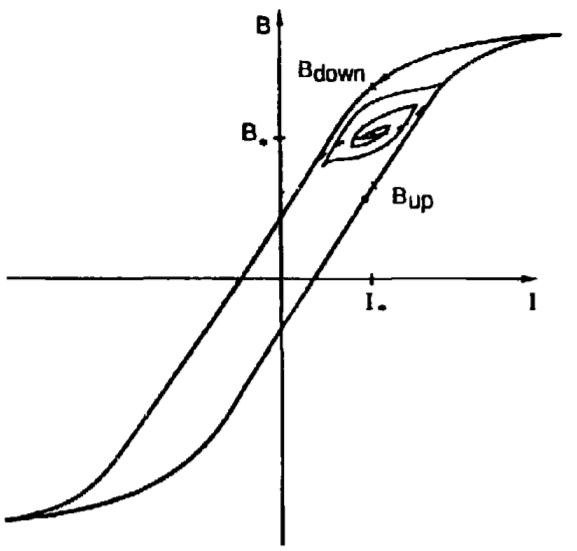
\includegraphics[width=0.7\textwidth]{Figures/CBETA_Multi-Pass_Commissioning/example_BI_curve.png}
\caption{}
\label{fig:example_BI_curve}
\end{figure}

The basic procedure is to repetitively alternate the current passed through the coils of the magnet around the tuning set point thereby increasing and decreasing the induced magnetic field. This shifts the position in the $B$--$H$ (or $B$--$I$) hysteresis curve upon which the magnet lies and instead leads to the magnet following its original $B$--$H$ curve. \textcolor{blue}{**Explanation needs a lot of work**} The original trialed procedure was based upon the procedure used for a series of quadrupoles at LCLS \cite{weidemann2010degaussing}.   

In order to increase reproducibility of the CBETA ERL configuration during commissioning a script was devised to combat the hysteresis effects by 'de-Gaussing' the magnets within the splitter lines. Only the splitter line magnets are chosen at this procedure is only applicable to electromagnets; the FFA magnets are permanent magnet quadrupoles and combined function magnets. 

\section{Multi-pass FFA Chromaticity Measurement}

\end{document}